\documentclass[]{article}
\usepackage{lmodern}
\usepackage[compact]{titlesec}
\usepackage{amssymb,amsmath}
\usepackage{ifxetex,ifluatex}
\usepackage{fixltx2e} % provides \textsubscript
\ifnum 0\ifxetex 1\fi\ifluatex 1\fi=0 % if pdftex
  \usepackage[T1]{fontenc}
  \usepackage[utf8]{inputenc}
\else % if luatex or xelatex
  \ifxetex
    \usepackage{mathspec}
  \else
    \usepackage{fontspec}
  \fi
  \defaultfontfeatures{Ligatures=TeX,Scale=MatchLowercase}
\fi
% use upquote if available, for straight quotes in verbatim environments
\IfFileExists{upquote.sty}{\usepackage{upquote}}{}
% use microtype if available
\IfFileExists{microtype.sty}{%
\usepackage{microtype}
\UseMicrotypeSet[protrusion]{basicmath} % disable protrusion for tt fonts
}{}
\usepackage[margin=1in]{geometry}
\usepackage{hyperref}
\hypersetup{unicode=true,
            pdftitle={Assignment 1: Moneyball Baseball Problem},
            pdfauthor={Darryl Buswell},
            pdfborder={0 0 0},
            breaklinks=true}
\urlstyle{same}  % don't use monospace font for urls
\usepackage{longtable,booktabs}
\usepackage{graphicx,grffile}
\makeatletter
\def\maxwidth{\ifdim\Gin@nat@width>\linewidth\linewidth\else\Gin@nat@width\fi}
\def\maxheight{\ifdim\Gin@nat@height>\textheight\textheight\else\Gin@nat@height\fi}
\makeatother
% Scale images if necessary, so that they will not overflow the page
% margins by default, and it is still possible to overwrite the defaults
% using explicit options in \includegraphics[width, height, ...]{}
\setkeys{Gin}{width=\maxwidth,height=\maxheight,keepaspectratio}
\IfFileExists{parskip.sty}{%
\usepackage{parskip}
}{% else
\setlength{\parindent}{0pt}
\setlength{\parskip}{6pt plus 2pt minus 1pt}
}
\setlength{\emergencystretch}{3em}  % prevent overfull lines
\providecommand{\tightlist}{%
  \setlength{\itemsep}{0pt}\setlength{\parskip}{0pt}}
\setcounter{secnumdepth}{0}
% Redefines (sub)paragraphs to behave more like sections
\ifx\paragraph\undefined\else
\let\oldparagraph\paragraph
\renewcommand{\paragraph}[1]{\oldparagraph{#1}\mbox{}}
\fi
\ifx\subparagraph\undefined\else
\let\oldsubparagraph\subparagraph
\renewcommand{\subparagraph}[1]{\oldsubparagraph{#1}\mbox{}}
\fi

%%% Use protect on footnotes to avoid problems with footnotes in titles
\let\rmarkdownfootnote\footnote%
\def\footnote{\protect\rmarkdownfootnote}

%%% Change title format to be more compact
\usepackage{titling}

% Create subtitle command for use in maketitle
\newcommand{\subtitle}[1]{
  \posttitle{
    \begin{center}\large#1\end{center}
    }
}

\setlength{\droptitle}{-2em}
  \title{Assignment 1: Moneyball Baseball Problem}
  \pretitle{\vspace{\droptitle}\centering\huge}
  \posttitle{\par}
\subtitle{MSPA PREDICT 411-DL-SEC56}
  \author{Darryl Buswell}
  \preauthor{\centering\large\emph}
  \postauthor{\par}
  \date{}
  \predate{}\postdate{}

\begin{document}
\maketitle

\section{1 Introduction}\label{introduction}

This document presents results of the first assignment for the Masters
of Science in Predictive Analytics course: PREDICT 411. This assessment
required the student to build an Ordinary Least Squares (OLS) regression
model which is able to predict the number of wins for a baseball team.
In order to find the `best' predictive model, this assessment manually
specified one regression model and employed two automated variable
selection techniques with the resultant model specifications assessed
over a range of performance criteria. Automated variable selection
techniques included the adjusted R Squared and stepwise variable
selection methods, which were assessed using metrics such as Mean Square
Error (MSE), Mean Absolute Error (MAE), Adjusted R-square, Akaike
Information Criterion (AIC) and Bayesian Information Criterion (BIC). A
final model was selected and used to generate a range of prediction
labels based on a test set of data.

As a bonus, this assessment employed Principal Component Analysis (PCA)
as a method of dimensionality reduction for regression analysis. PCA is
initially performed on the dataset in order to derive a set of
components. A regression model is then fitted which makes use of the
principle components for its set of predictor variables. Finally, an
assessment of the model is made, with a focus on whether using principle
components for predictor variables results in an improvement in either
goodness-of-fit or model performance.

\section{2 Data}\label{data}

The dataset contains variables which focus on performance statistics for
baseball teams over the years 1871 to 2006. Each record details the
performance of a team for any given year, with all statistics adjusted
to match the performance of a 162 game season. For this assessment, two
datasets have been provided, one is a training set of data, which is
comprised of 2,276 observations. The second is a testing data set of
data, which is comprised of 259 observations.

At a first pass, it seems the dataset has quite a large amount of scope.
There are variables tracking a number of gameplay attributes, including
those related to batter performance, pitcher performance and gameplay
outcomes. The below table shows a list of variables included in the
original dataset. A proposed effect on the response variable is also
shown for each.

\paragraph{Table 2.1: Variable
Descriptions}\label{table-2.1-variable-descriptions}

\begin{longtable}[]{@{}lll@{}}
\toprule
Variable & Definition & Proposed Effect on Wins\tabularnewline
\midrule
\endhead
TARGET\_WINS & Target wins &\tabularnewline
TEAM\_BATTING\_H & Base Hits by batters & Positive\tabularnewline
TEAM\_BATTING\_2B & Doubles by batters & Positive\tabularnewline
TEAM\_BATTING\_3B & Triples by batters & Positive\tabularnewline
TEAM\_BATTING\_HR & Homeruns by batters & Positive\tabularnewline
TEAM\_BATTING\_BB & Walks by batters & Positive\tabularnewline
TEAM\_BATTING\_SO & Strikeouts by batters & Negative\tabularnewline
TEAM\_BASERUN\_SB & Stolen bases & Positive\tabularnewline
TEAM\_BASERUN\_CS & Caught stealing & Negative\tabularnewline
TEAM\_BATTING\_HBP & Batters hit by pitch & Positive\tabularnewline
TEAM\_PITCHING\_H & Hits allowed & Negative\tabularnewline
TEAM\_PITCHING\_HR & Homeruns allowed & Negative\tabularnewline
TEAM\_PITCHING\_BB & Walks allowed & Negative\tabularnewline
TEAM\_PITCHING\_SO & Strikeouts by pitchers & Positive\tabularnewline
TEAM\_FIELDING\_E & Errors & Negative\tabularnewline
TEAM\_FIELDING\_DP & Double Plays & Positive\tabularnewline
\bottomrule
\end{longtable}

It is worth noting the dataset has quite a long span (from 1871 to
2006). As such, the dataset may indeed suffer from consistency issues.
For example, there may have been changes as to how the data for each
variable was collected over this period, or even changes to the nature
of what each variable is to represent. Unfortunately, the dataset does
not include a variable to allow observations to be identified by time,
which limits our ability to deal with this issue.

\section{3 Data Exploration}\label{data-exploration}

Prior to performing any regression analysis, a number of data
exploration routines are conducted. These routines allow us to gain an
understanding of any potential limitations of the dataset, including
identifying variables which have missing observations, outlier
observations, or those variables which may benefit from transformation.

\subsection{3.1 Univariate Data
Analysis}\label{univariate-data-analysis}

A review of the dataset shows that each variable is of continuous type
with varying statistical properties. Summary statistics for each
variable is shown in the table below.

\paragraph{Table 3.1.1: Data
Statistics}\label{table-3.1.1-data-statistics}

\begin{longtable}[]{@{}lllllll@{}}
\toprule
Variable & Minimum & Maximum & Mean & Std Dev & N Miss &
N\tabularnewline
\midrule
\endhead
TARGET\_WINS & 0 & 146 & 80.7908612 & 15.7521525 & 0 &
2276\tabularnewline
TEAM\_BATTING\_H & 891 & 2554 & 1469.27 & 144.5911954 & 0 &
2276\tabularnewline
TEAM\_BATTING\_2B & 69 & 458 & 241.2469244 & 46.8014146 & 0 &
2276\tabularnewline
TEAM\_BATTING\_3B & 0 & 223 & 55.25 & 27.938557 & 0 &
2276\tabularnewline
TEAM\_BATTING\_HR & 0 & 264 & 99.6120387 & 60.546872 & 0 &
2276\tabularnewline
TEAM\_BATTING\_BB & 0 & 878 & 501.5588752 & 122.6708615 & 0 &
2276\tabularnewline
TEAM\_BATTING\_SO & 0 & 1399 & 735.6053358 & 248.5264177 & 102 &
2174\tabularnewline
TEAM\_BASERUN\_SB & 0 & 697 & 124.7617716 & 87.791166 & 131 &
2145\tabularnewline
TEAM\_BASERUN\_CS & 0 & 201 & 52.8038564 & 22.9563376 & 772 &
1504\tabularnewline
TEAM\_BATTING\_HBP & 29 & 95 & 59.3560209 & 12.9671225 & 2085 &
191\tabularnewline
TEAM\_PITCHING\_H & 1137 & 30132 & 1779.21 & 1406.84 & 0 &
2276\tabularnewline
TEAM\_PITCHING\_HR & 0 & 343 & 105.698594 & 61.2987469 & 0 &
2276\tabularnewline
TEAM\_PITCHING\_BB & 0 & 3645 & 553.0079086 & 166.3573617 & 0 &
2276\tabularnewline
TEAM\_PITCHING\_SO & 0 & 19278 & 817.7304508 & 553.0850315 & 102 &
2174\tabularnewline
TEAM\_FIELDING\_E & 65 & 1898 & 246.4806678 & 227.7709724 & 0 &
2276\tabularnewline
TEAM\_FIELDING\_DP & 52 & 228 & 146.3879397 & 26.2263853 & 286 &
1990\tabularnewline
\bottomrule
\end{longtable}

What becomes immediately obvious is that a number of variables suffer
from a large amount of missing observations. TEAM\_BATTING\_HBP in
particular, includes only 191 observations, which is less than 10\% of
the total number of observations recorded for the wider dataset. While
the remaining variables with missing observations may benefit from some
form of imputation, this variable will instead be excluded from the
analysis completely.

\newpage

\paragraph{Figure 3.1.1 Histogram: Team Batting
2B}\label{figure-3.1.1-histogram-team-batting-2b}

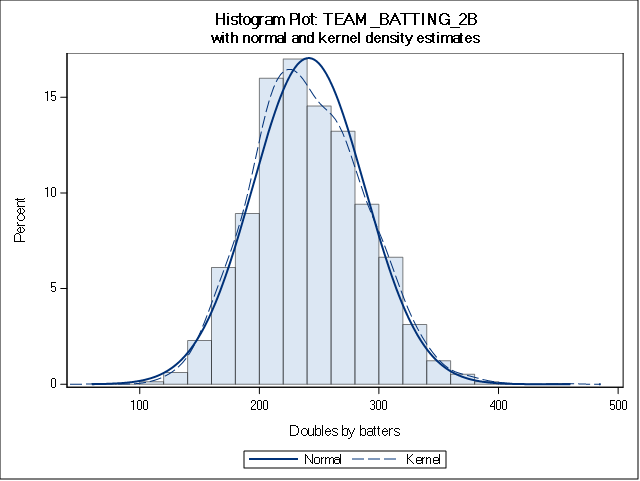
\includegraphics[height=3.95833in]{images/hist_team_batting_2b.png}

\paragraph{Figure 3.1.2 Box Plot: Team Batting
2B}\label{figure-3.1.2-box-plot-team-batting-2b}

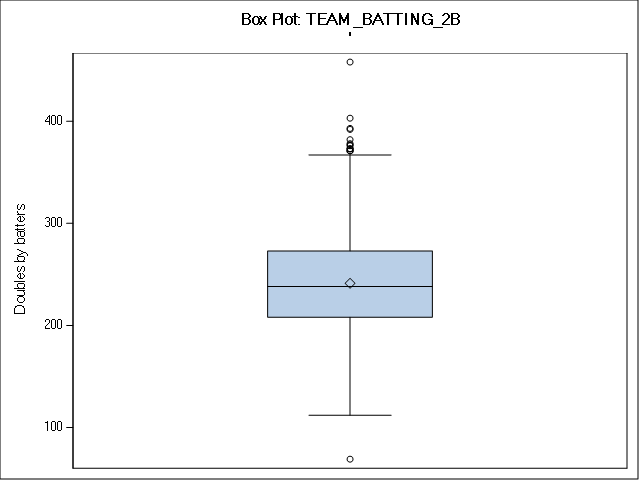
\includegraphics[height=3.95833in]{images/box_team_batting_2b.png}

\newpage

\paragraph{Figure 3.1.3 Histogram: Team Batting
3B}\label{figure-3.1.3-histogram-team-batting-3b}

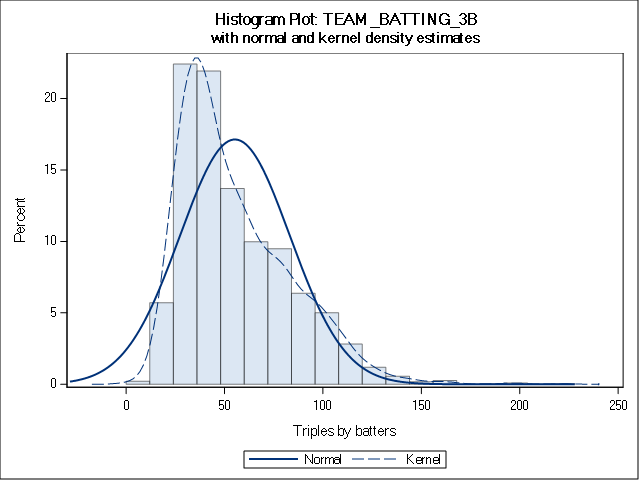
\includegraphics[height=3.95833in]{images/hist_team_batting_3b.png}

\paragraph{Figure 3.1.4 Box Plot: Team Batting
3B}\label{figure-3.1.4-box-plot-team-batting-3b}

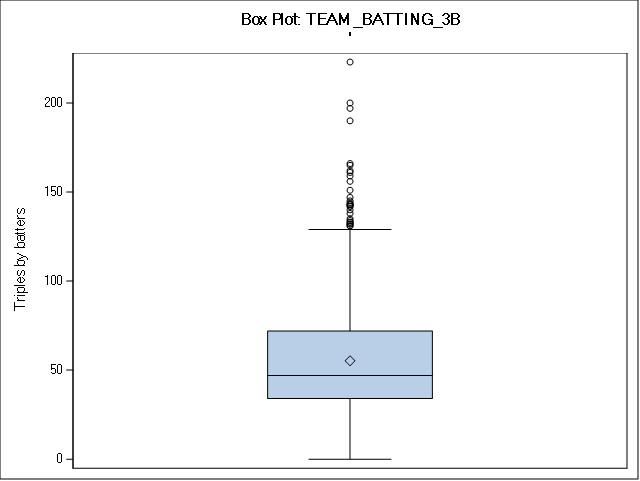
\includegraphics[height=3.95833in]{images/box_team_batting_3b.png}

\newpage

\paragraph{Figure 3.1.5 Histogram: Team Batting
HR}\label{figure-3.1.5-histogram-team-batting-hr}

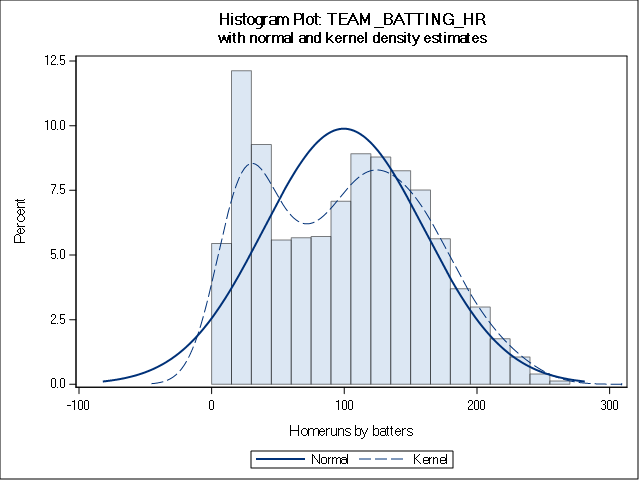
\includegraphics[height=3.95833in]{images/hist_team_batting_hr.png}

\paragraph{Figure 3.1.6 Box Plot: Team Batting
HR}\label{figure-3.1.6-box-plot-team-batting-hr}

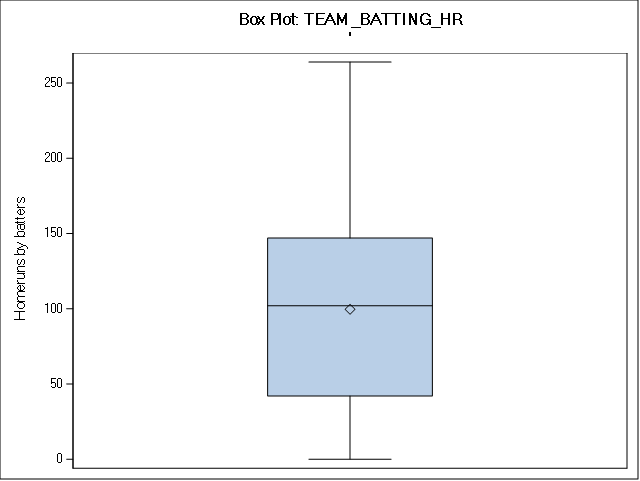
\includegraphics[height=3.95833in]{images/box_team_batting_hr.png}

\newpage

We can also use a combination of histogram and box plots in order to
gain a greater understanding of each variable included within the
dataset. Histogram and box plots were generated and reviewed for all
variables, however with plots for only three variables were selected for
further discussion. We can see that TEAM\_BATTING\_2B, has a normal
shaped distribution, and minimal outliers. However, there are variables
within the dataset such as TEAM\_BATTING\_3B which have a heavy skew. In
this case, the positive skewed distribution also carries a number of
outlier observations. Even more concerning are variables such as
TEAM\_BATTING\_HR, which seem to have quite a non-normal shaped
distribution. In this case, observations seem to collect around both a
low and high value, resulting in a bimodal shaped distribution.

\subsection{3.2 Bivariate Data Analysis}\label{bivariate-data-analysis}

Since we intend on building a prediction model for target wins, we have
an interest in those variables which have explanatory power over this
variable. As such, we can use the SAS procedure `corr' to see if there
are any variables that have a high Pearson correlation coefficient and
low \(p\)-value in relation to our response variable.

\paragraph{Table 3.2.1: Data
Correlations}\label{table-3.2.1-data-correlations}

\begin{longtable}[]{@{}lll@{}}
\toprule
Variable & Correlation & Proposed Effect on Wins\tabularnewline
\midrule
\endhead
TEAM\_BATTING\_H & 0.38877 & Positive\tabularnewline
TEAM\_BATTING\_2B & 0.28910 & Positive\tabularnewline
TEAM\_BATTING\_3B & 0.14261 & Positive\tabularnewline
TEAM\_BATTING\_HR & 0.17615 & Positive\tabularnewline
TEAM\_BATTING\_BB & 0.23256 & Positive\tabularnewline
TEAM\_BATTING\_SO & -0.03175 & Negative\tabularnewline
TEAM\_BASERUN\_SB & 0.13514 & Positive\tabularnewline
TEAM\_BASERUN\_CS & 0.02240 & Negative\tabularnewline
TEAM\_PITCHING\_H & -0.10994 & Negative\tabularnewline
TEAM\_PITCHING\_HR & 0.18901 & Negative\tabularnewline
TEAM\_PITCHING\_BB & 0.12417 & Negative\tabularnewline
TEAM\_PITCHING\_SO & -0.07844 & Positive\tabularnewline
TEAM\_FIELDING\_E & -0.17648 & Negative\tabularnewline
TEAM\_FIELDING\_DP & -0.03485 & Positive\tabularnewline
\bottomrule
\end{longtable}

None of the variables are reported to have a particularly strong
positive or negative correlation coefficient with the response variable,
with the greatest absolute correlation being reported by `base hits by
batters' and `doubles by batters' at 0.39 and 0.29 respectively. We also
observe that a number of variables polarity of correlation coefficient
does not match the proposed effect on wins. We will take note of these
variables, as they may have less justification for inclusion in any
regressions which are manually specified.

We can also use scatter plots with a Locally Estimated Scatter Plot
Smoother (LOESS) overlay to further explore the relationship between the
response variable and each predictor variable. Scatter plots for a
collection of variables against the response variable were generated and
reviewed, however only two of these plots were selected for further
discussion below. We can see from the plots that both TEAM\_BASERUN\_CS
and TEAM\_BATTING\_HR do indeed have little positive or negative
relation with TARGET\_WINS. It is worth noting that while many variables
such as TEAM\_BASERUN\_CS are prone to outlier observations which
results in the appearance of a tight collection of observations on
scatterplots, there are a selection of variables such as
TEAM\_BATTING\_HR who suffer less from outliers which results in a more
uniform pattern over scatter plots.

\newpage

\paragraph{Figure 3.2.1 Scatter: Team Baserun
CS}\label{figure-3.2.1-scatter-team-baserun-cs}

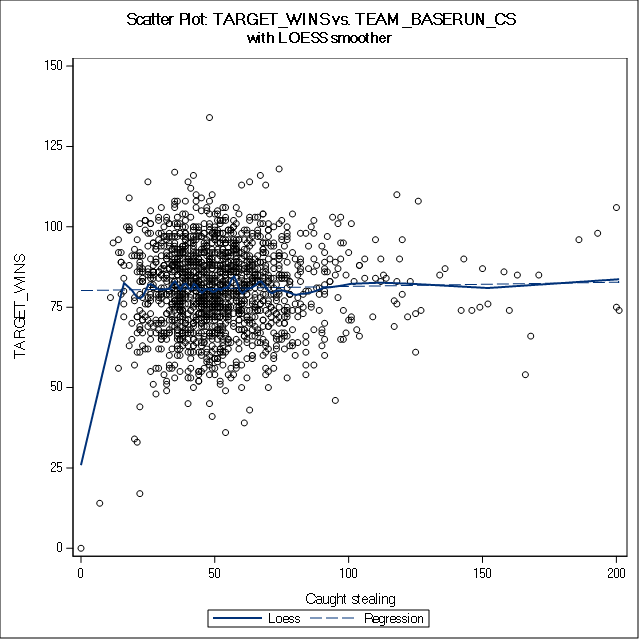
\includegraphics[height=3.95833in]{images/scatter_team_baserun_cs.png}

\paragraph{Figure 3.2.3 Scatter: Team Batting
HR}\label{figure-3.2.3-scatter-team-batting-hr}

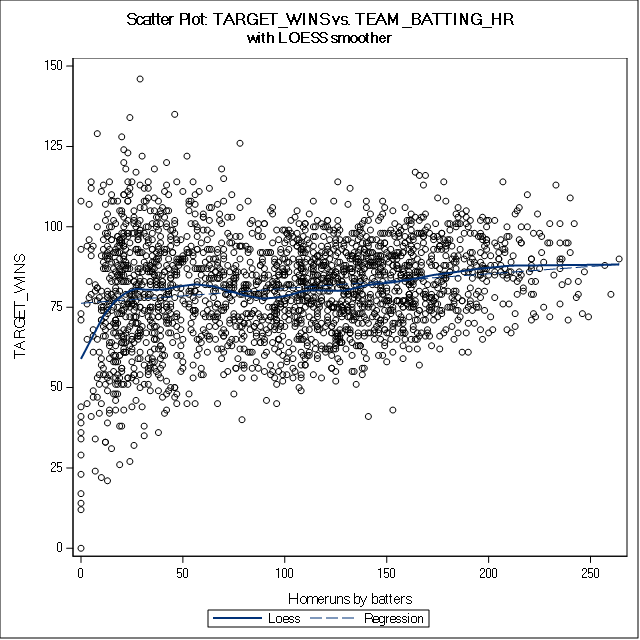
\includegraphics[height=3.95833in]{images/scatter_team_batting_hr.png}

\section{4 Data Preparation}\label{data-preparation}

From an observation of each univariate and bivariate plot, we have
identified that the majority of variables do in-fact suffer from outlier
observations. In fact, only TEAM\_BATTING\_HR, TEAM\_BATTING\_SO and
TEAM\_PITCHING\_HR were shown to have minimal outlier observations, with
variables such as TEAM\_PITCHING\_H, TEAM\_FIELDING\_E and
TEAM\_BASERUN\_SB having the greatest number of outliers. A review of
the percentiles for each variable confirms this, with a rather large gap
between min, max and the 1st and 99th percentile respectively. A summary
of percentiles for each variable can be found in the table below.

\paragraph{Table 4.1: Quantiles
Summary}\label{table-4.1-quantiles-summary}

\begin{longtable}[]{@{}llllllllllll@{}}
\toprule
Variable & Max & 0.99 & 0.95 & 0.9 & Q3 & Med & Q1 & 0.1 & 0.05 & 0.01 &
Min\tabularnewline
\midrule
\endhead
TARGET\_WINS & 146 & 114 & 104 & 100 & 92 & 82 & 71 & 61 & 54 & 38 &
0\tabularnewline
TEAM\_BATTING\_H & 2554 & 1950 & 1696 & 1636 & 1537.5 & 1454 & 1383 &
1315 & 1280 & 1188 & 891\tabularnewline
TEAM\_BATTING\_2B & 458 & 352 & 320 & 303 & 273 & 238 & 208 & 182 & 167
& 141 & 69\tabularnewline
TEAM\_BATTING\_3B & 223 & 134 & 108 & 96 & 72 & 47 & 34 & 27 & 23 & 17 &
0\tabularnewline
TEAM\_BATTING\_HR & 264 & 235 & 199 & 180 & 147 & 102 & 42 & 20 & 14 & 4
& 0\tabularnewline
TEAM\_BATTING\_BB & 878 & 755 & 671 & 635 & 580 & 512 & 451 & 363 & 246
& 79 & 0\tabularnewline
TEAM\_BATTING\_SO & 1399 & 1193 & 1104 & 1049 & 930 & 750 & 548 & 421 &
359 & 67 & 0\tabularnewline
TEAM\_BASERUN\_SB & 697 & 439 & 302 & 231 & 156 & 101 & 66 & 44 & 35 &
23 & 0\tabularnewline
TEAM\_BASERUN\_CS & 201 & 143 & 91 & 77 & 62 & 49 & 38 & 30 & 24 & 16 &
0\tabularnewline
TEAM\_PITCHING\_H & 30132 & 7093 & 2563 & 2059 & 1683 & 1518 & 1419 &
1356 & 1316 & 1244 & 1137\tabularnewline
TEAM\_PITCHING\_HR & 343 & 244 & 210 & 187 & 150 & 107 & 50 & 25 & 18 &
8 & 0\tabularnewline
TEAM\_PITCHING\_BB & 3645 & 924 & 757 & 694 & 611 & 536.5 & 476 & 417 &
377 & 237 & 0\tabularnewline
TEAM\_PITCHING\_SO & 19278 & 1474 & 1173 & 1095 & 968 & 813.5 & 615 &
490 & 420 & 205 & 0\tabularnewline
TEAM\_FIELDING\_E & 1898 & 1237 & 716 & 542 & 249.5 & 159 & 127 & 109 &
100 & 86 & 65\tabularnewline
TEAM\_FIELDING\_DP & 228 & 204 & 186 & 178 & 164 & 149 & 131 & 109 & 98
& 79 & 52\tabularnewline
\bottomrule
\end{longtable}

We do not know at this point whether these outlier observations have
predictive power over TARGET\_WINS. To understand this, one option may
be to conduct a simple Ordinary Least Squares (OLS) for each variable
against our response variable and observe the residuals of each. For
this assessment however, we have elected to instead generate a trimmed
copy of all variables, and will rely on automated variable selection
routines to identify those variables which demonstrate the greatest
predictive power. Such a method will help reduce the amount of selective
bias introduced by the analyst.

From a review of both the univariate plots in the previous section as
well as the quantile summaries above, we have elected to generate
trimmed copies of each variable by their 99th percentile. Although the
inclusion of additional trimmed variables is an option, at this stage we
prefer to minimize the amount of adjusted variable copies introduced
into the dataset. Trimmed variables include the suffix '\_T99'.

Following introducing copies of trimmed variables, we then look towards
imputing values for missing observations. By recalculating statistical
measures for each variable after trimming, we are able to avoid imputing
skewed values for those variables which have been trimmed into each
variable. For this assessment, we generate new imputed variables based
on that variable's median value. Note that in order to simplify the SAS
logic used for this assessment, all variables will include the suffix
'\_IME', however only those variables shown to have missing observations
in the previous section have actually received imputation.

As a final step in our data preparation routine, we perform a natural
logarithm transformation of each variable. Variables which have been
transformed include the suffix '\_LN'. Such a transformation will help
penalize extreme values and may provide an improved fit within
subsequent regression models.

\section{5 Model Development}\label{model-development}

For this section, we build three linear regression models. For the first
`Subjective Model', variables have been retained based our opinion of
which would likely have the greatest relevance towards predicting wins.
The remaining two models are specified according to automated variable
selection techniques. The `Adjusted R-squared Selection Model', which
uses the maximum improvement technique for variable selection. And
finally, the `Stepwise Selection Model' which uses the stepwise
selection technique for variable selection.

\subsection{5.1 Model 1: Subjective
Model}\label{model-1-subjective-model}

For the Subjective Model (Model\_Subj), we include only those variables
which were shown to produce a correlation coefficient against the
response variable which was aligned with our proposed effect. We build
on this by including missing variable flags for those variables which
were shown to have missing variables, and outlier flags for those
variables which were shown to have a large amount of outliers. Finally,
we removed any variables from this specification which were found to be
highly insignificant.

Parameter estimates for the Model\_Subj are shown below.

\paragraph{Table 5.1.1: Subjective Model Parameter Estimates (Training
Set)}\label{table-5.1.1-subjective-model-parameter-estimates-training-set}

\begin{longtable}[]{@{}lllllll@{}}
\toprule
Variable & DF & Par. Est. & Par. S.E. & t Value & \$\text{Pr}
\textgreater{} & t\tabularnewline
\midrule
\endhead
Intercept & 1 & 3.16454 & 5.617 & 0.56 & 0.5733 & 0\tabularnewline
TEAM\_BATTING\_H\_IME & 1 & 0.04876 & 0.00413 & 11.82 & \textless{}.0001
& 3.71652\tabularnewline
TEAM\_BATTING\_2B\_IME & 1 & -0.03895 & 0.01065 & -3.66 & 0.0003 &
2.68623\tabularnewline
TEAM\_BATTING\_3B\_IME & 1 & 0.08737 & 0.01949 & 4.48 & \textless{}.0001
& 3.02755\tabularnewline
TEAM\_BATTING\_HR\_IME & 1 & 0.06472 & 0.0113 & 5.73 & \textless{}.0001
& 4.96995\tabularnewline
TEAM\_BATTING\_BB\_IME & 1 & 0.02307 & 0.00387 & 5.96 & \textless{}.0001
& 2.37525\tabularnewline
TEAM\_BATTING\_SO\_IME & 1 & -0.00891 & 0.00264 & -3.37 & 0.0008 &
4.23806\tabularnewline
TEAM\_BASERUN\_SB\_IME & 1 & 0.06231 & 0.00529 & 11.78 &
\textless{}.0001 & 2.02626\tabularnewline
TEAM\_PITCHING\_H\_IME & 1 & 0.0012 & 0.00036487 & 3.28 & 0.0011 &
3.2279\tabularnewline
TEAM\_FIELDING\_E\_IME & 1 & -0.05495 & 0.00357 & -15.4 &
\textless{}.0001 & 7.04413\tabularnewline
TEAM\_BATTING\_SO\_MF & 1 & 9.90691 & 1.61891 & 6.12 & \textless{}.0001
& 1.30858\tabularnewline
TEAM\_BASERUN\_SB\_MF & 1 & 36.73709 & 2.23367 & 16.45 &
\textless{}.0001 & 3.02158\tabularnewline
TEAM\_BATTING\_3B\_OF & 1 & -4.02422 & 2.56594 & -1.57 & 0.117 &
1.16292\tabularnewline
TEAM\_PITCHING\_H\_OF & 1 & 3.98635 & 2.71559 & 1.47 & 0.1423 &
1.63274\tabularnewline
TEAM\_FIELDING\_E\_OF & 1 & 4.8098 & 2.73651 & 1.76 & 0.079 &
1.41879\tabularnewline
\bottomrule
\end{longtable}

For Model\_Subj, the majority of coefficient estimates have significant
p-values at the 95\% level, allowing us to reject the null hypothesis
and conclude that each have non-zero coefficients. The only exceptions
are the outlier flag variables, TEAM\_BATTING\_3B\_OF,
TEAM\_PITCHING\_H\_OF and TEAM\_FIELDING\_E\_OF. We also note that the
polarity of estimate for the majority of coefficients seems reasonable,
with the only exceptions being TEAM\_BATTING\_2B\_IME and
TEAM\_PITCHING\_H\_IME. We also note the magnitude of the coefficient
estimate for each of the non-flag variables is quite small, suggesting
only a marginal expected change in wins based on a unit change in each.
Finally, we note that the VIF for the majority of predictor variables is
less than five suggesting little to moderate correlation between
predictors.

Goodness-of-fit information for Model\_Subj is shown below.

\paragraph{Table 5.1.2: Subjective Model Analysis of Variance (Training
Set)}\label{table-5.1.2-subjective-model-analysis-of-variance-training-set}

\begin{longtable}[]{@{}llllll@{}}
\toprule
Source & DF & Sum of Squares & Mean Square & F Value & Pr \textgreater{}
F\tabularnewline
\midrule
\endhead
Model & 14 & 166986 & 11928 & 79.40 & \textless{}.0001\tabularnewline
Error & 1547 & 232393 & 150.22183 & &\tabularnewline
Corrected Total & 1561 & 399379 & & &\tabularnewline
\bottomrule
\end{longtable}

The model has reported a large F-value suggesting that the observations
and regression differ from the grand mean. Likewise, the F-value has a
highly significant p-value under the null hypothesis that there is no
linear relationship between the predictor and response variable.

Model performance statistics over the training set for Model\_Subj are
shown below.

\paragraph{Table 5.1.3: Subjective Model Performance Metrics (Training
Set)}\label{table-5.1.3-subjective-model-performance-metrics-training-set}

\begin{longtable}[]{@{}llll@{}}
\toprule
Measure & Value & Measure & Value\tabularnewline
\midrule
\endhead
MSE & 150.22183 & R-Square & 0.4181\tabularnewline
MAE & 9.71342 & Adj R-Sq & 0.4128\tabularnewline
Root MSE & 12.25650 & C(p) & 15.0000\tabularnewline
Dependent Mean & 80.57875 & AIC & 7843.8481\tabularnewline
Coeff Var & 15.21059 & BIC & 7846.1388\tabularnewline
\bottomrule
\end{longtable}

The R-square value above suggests that Model\_Subj explains
\textasciitilde{}42\% of the variability in TARGET\_WINS using each of
the included predictor variables. The adjusted R-squared value also
indicates a similar level of explanatory power. The AIC and BIC are also
reported above. Both AIC and BIC form a model selection criteria which
look to assess goodness of fit of the model. These metrics will be used
to assess the above model against models formed from alternative
automated selection techniques below.

Model performance statistics over the training set for Model\_Subj are
shown below.

\paragraph{Table 5.1.4: Subjective Model Performance Metrics (Test
Set)}\label{table-5.1.4-subjective-model-performance-metrics-test-set}

\begin{longtable}[]{@{}llll@{}}
\toprule
Measure & Value & Measure & Value\tabularnewline
\midrule
\endhead
MSE & 146.95376 & R-Square & 0.3646\tabularnewline
MAE & 9.29372 & Adj R-Sq & 0.3770\tabularnewline
Root MSE & 12.12245 & C(p) & 15.0000\tabularnewline
Dependent Mean & 81.25490 & AIC & 3577.7844\tabularnewline
Coeff Var & 14.91904 & BIC & 3580.4273\tabularnewline
\bottomrule
\end{longtable}

From the table above, we can see that applying the same model
specification to the test set of data shows a slight reduction in MSE,
MAE and likewise, a reduction in reported R-Square and adjusted R-Square
values. Although we can also see a reduction in AIC and BIC, these
metrics are better suited to compare alternative model specifications
which have been assessed against the test set of data. Generally,
performance metrics for Model\_Subj have remained fairly consistent
between the training and test sets, suggesting that the model is able to
generalize over the test set of data.

\subsection{5.2 Model 2: AdjR2 Selection
Model}\label{model-2-adjr2-selection-model}

The adjusted R-squared selection technique finds subsets of independent
variables that `best' predict the dependent variable. `Best' is defined
by this technique as the model which produces the highest adjusted
R-squared value (Inc 2016). This technique is applied to the training
set of data, with the resulting model (Model\_AdjR2) shown below.

Parameter estimates for Model\_AdjR2 are shown below.

\paragraph{Table 5.2.1: Model AdjR2 Parameter Estimates (Training
Set)}\label{table-5.2.1-model-adjr2-parameter-estimates-training-set}

\begin{longtable}[]{@{}lllllll@{}}
\toprule
Variable & DF & Par. Est. & Par. S.E. & t Value & \$\text{Pr}
\textgreater{} & t\tabularnewline
\midrule
\endhead
Intercept & 1 & 4.03808 & 86.73687 & 0.05 & 0.9629 & 0\tabularnewline
TEAM\_BASERUN\_CS\_OF & 1 & 3.39374 & 1.01873 & 3.33 & 0.0009 &
2.6933\tabularnewline
TEAM\_BASERUN\_SB\_MF & 1 & 33.98348 & 2.12377 & 16 & \textless{}.0001 &
2.98107\tabularnewline
TEAM\_BATTING\_SO\_MF & 1 & 7.44002 & 1.73068 & 4.3 & \textless{}.0001 &
1.63211\tabularnewline
TEAM\_FIELDING\_DP\_MF & 1 & 6.18056 & 1.7548 & 3.52 & 0.0004 &
3.69955\tabularnewline
TEAM\_BASERUN\_SB\_IME & 1 & 0.0485 & 0.00553 & 8.76 & \textless{}.0001
& 2.41932\tabularnewline
TEAM\_BATTING\_2B\_T99\_IME & 1 & -0.25625 & 0.06227 & -4.12 &
\textless{}.0001 & 85.18334\tabularnewline
TEAM\_BATTING\_3B\_T99\_IME & 1 & 0.1575 & 0.01908 & 8.26 &
\textless{}.0001 & 2.71637\tabularnewline
TEAM\_BATTING\_BB\_IME & 1 & 0.02836 & 0.00365 & 7.77 & \textless{}.0001
& 2.30183\tabularnewline
TEAM\_BATTING\_H\_IME & 1 & 0.06498 & 0.00412 & 15.77 & \textless{}.0001
& 4.04579\tabularnewline
TEAM\_PITCHING\_HR\_IME & 1 & 0.04503 & 0.00987 & 4.56 &
\textless{}.0001 & 4.25924\tabularnewline
TEAM\_PITCHING\_SO\_T99\_IME & 1 & -0.04225 & 0.00806 & -5.24 &
\textless{}.0001 & 35.47802\tabularnewline
TEAM\_BATTING\_2B\_T99\_IME\_LN & 1 & 49.84735 & 14.86247 & 3.35 &
0.0008 & 86.28656\tabularnewline
TEAM\_BATTING\_H\_T99\_IME\_LN & 1 & -26.9484 & 7.31153 & -3.69 & 0.0002
& 3.9306\tabularnewline
TEAM\_FIELDING\_DP\_IME\_LN & 1 & -16.05367 & 2.26834 & -7.08 &
\textless{}.0001 & 1.96833\tabularnewline
TEAM\_FIELDING\_E\_IME\_LN & 1 & -23.64552 & 1.3426 & -17.61 &
\textless{}.0001 & 7.65474\tabularnewline
TEAM\_PITCHING\_SO\_T99\_IME\_LN & 1 & 25.16199 & 6.22459 & 4.04 &
\textless{}.0001 & 37.675\tabularnewline
\bottomrule
\end{longtable}

For Model\_AdjR2, all coefficient estimates have significant p-values at
the 95\% level, allowing us to reject the null hypothesis for each
estimate and conclude that each have non-zero coefficients. We also note
that the polarity of estimate for many of coefficients seems reasonable,
with the exceptions being TEAM\_BATTING\_2B\_T99\_IME,
TEAM\_BATTING\_BB\_IME, TEAM\_PITCHING\_H, TEAM\_FIELDING\_DP\_IME\_LN
and TEAM\_PITCHING\_SO\_T99\_IME\_LN. Unfortunately, a number of
variables are included which have VIF's greater than 10, suggesting a
high amount of correlation with the remaining predictors.

Goodness-of-fit information for Model\_AdjR2 is shown below.

\paragraph{Table 5.2.2: Model AdjR2 Analysis of Variance (Training
Set)}\label{table-5.2.2-model-adjr2-analysis-of-variance-training-set}

\begin{longtable}[]{@{}llllll@{}}
\toprule
Source & DF & Sum of Squares & Mean Square & F Value & Pr \textgreater{}
F\tabularnewline
\midrule
\endhead
Model & 16 & 186712 & 11669 & 84.78 & \textless{}.0001\tabularnewline
Error & 1545 & 212667 & 137.64865 & &\tabularnewline
Corrected Total & 1561 & 399379 & & &\tabularnewline
\bottomrule
\end{longtable}

The model has reported a large F-value suggesting that the observations
and regression differ from the grand mean. Likewise, the F-value has a
highly significant p-value under the null hypothesis that there is no
linear relationship between the predictor and response variable.

Model performance statistics over the training set for Model\_AdjR2 are
shown below.

\paragraph{Table 5.2.3: Model AdjR2 Performance Metrics (Training
Set)}\label{table-5.2.3-model-adjr2-performance-metrics-training-set}

\begin{longtable}[]{@{}llll@{}}
\toprule
Measure & Value & Measure & Value\tabularnewline
\midrule
\endhead
MSE & 137.64865 & R-Square & 0.4675\tabularnewline
MAE & 9.25776 & Adj R-Sq & 0.462\tabularnewline
Root MSE & 11.73238 & C(p) & 17\tabularnewline
Dependent Mean & 80.57875 & AIC & 7709.2951\tabularnewline
Coeff Var & 14.56014 & BIC & 7711.669\tabularnewline
\bottomrule
\end{longtable}

The R-square value above suggests that Model\_AdjR2 explains
\textasciitilde{}47\% of the variability in TARGET\_WINS using each of
the included predictor variables. The adjusted R-squared value for this
specification is slightly higher (superior) than that reported for
Model\_Subj (0.4128), and its AIC and BIC are slightly lower (superior)
than those reported for Model\_Subj (7843.8481 and 7846.1388
respectively). These metrics suggest that Model\_AdjR2 may have a
slightly better fit over the training set of data compared to
Model\_Subj.

Model performance statistics over the test set for Model\_AdjR2 are
shown below.

\paragraph{Table 5.2.4: Model AdjR2 Performance Metrics (Test
Set)}\label{table-5.2.4-model-adjr2-performance-metrics-test-set}

\begin{longtable}[]{@{}llll@{}}
\toprule
Measure & Value & Measure & Value\tabularnewline
\midrule
\endhead
MSE & 137.76292 & R-Square & 0.4177\tabularnewline
MAE & 9.03843 & Adj R-Sq & 0.4043\tabularnewline
Root MSE & 11.73725 & C(p) & 17\tabularnewline
Dependent Mean & 81.2549 & AIC & 3533.6258\tabularnewline
Coeff Var & 14.44497 & BIC & 3536.4539\tabularnewline
\bottomrule
\end{longtable}

Performance metrics for Model\_AdjR2 have remained fairly consistent
between the training and test sets. This suggests that the model is able
to generalize over the test set of data.

\subsection{5.3 Model 3: Stepwise
Selection}\label{model-3-stepwise-selection}

The stepwise technique is a modification of the forward-selection
technique. It differs in that variables already in the model do not
necessarily remain in the model (D. Montgomery 2012). For this
technique, we elected to use a SLENTRY value of 0.02, which indicates
that variables should only be added to the specification if they have a
significance level (p-value) of less than 2\%, and also elected to use a
SLSTAY value of 0.02, which indicates that variables should not be
removed from the specification if they have a significance level
(p-value) less than 2\%. This technique is applied to the training set
of data, with the resulting model (Model\_S) shown below.

Parameter estimates for Model\_S are shown below.

\paragraph{Table 5.3.1: Stepwise Selection Model Parameter Estimates
(Training
Set)}\label{table-5.3.1-stepwise-selection-model-parameter-estimates-training-set}

\begin{longtable}[]{@{}lllllll@{}}
\toprule
Variable & DF & Par. Est. & Par. S.E. & t Value & \$\text{Pr}
\textgreater{} & t\tabularnewline
\midrule
\endhead
Intercept & 1 & 266.4722 & 21.59628 & 12.34 & \textless{}.0001 &
0\tabularnewline
TEAM\_BASERUN\_CS\_OF & 1 & 3.44889 & 1.03252 & 3.34 & 0.0009 &
2.69668\tabularnewline
TEAM\_BASERUN\_SB\_IME & 1 & 0.05721 & 0.00546 & 10.47 &
\textless{}.0001 & 2.2965\tabularnewline
TEAM\_BASERUN\_SB\_MF & 1 & 34.88631 & 2.05252 & 17 & \textless{}.0001 &
2.71393\tabularnewline
TEAM\_BATTING\_3B\_T99\_IME & 1 & 0.15324 & 0.01927 & 7.95 &
\textless{}.0001 & 2.70108\tabularnewline
TEAM\_BATTING\_BB\_IME & 1 & 0.05204 & 0.00626 & 8.32 & \textless{}.0001
& 6.6007\tabularnewline
TEAM\_BATTING\_H\_IME & 1 & 0.05862 & 0.00394 & 14.89 & \textless{}.0001
& 3.59982\tabularnewline
TEAM\_BATTING\_H\_T99\_IME & 1 & -0.02893 & 0.00476 & -6.08 &
\textless{}.0001 & 3.59958\tabularnewline
TEAM\_BATTING\_SO\_IME & 1 & -0.01576 & 0.00244 & -6.46 &
\textless{}.0001 & 3.83262\tabularnewline
TEAM\_BATTING\_SO\_MF & 1 & 7.6899 & 1.69006 & 4.55 & \textless{}.0001 &
1.51701\tabularnewline
TEAM\_FIELDING\_DP\_IME\_LN & 1 & -14.46299 & 2.21211 & -6.54 &
\textless{}.0001 & 1.82458\tabularnewline
TEAM\_FIELDING\_DP\_OF & 1 & 4.45505 & 1.50274 & 2.96 & 0.0031 &
2.89485\tabularnewline
TEAM\_FIELDING\_E\_IME\_LN & 1 & -22.62866 & 1.41822 & -15.96 &
\textless{}.0001 & 8.32515\tabularnewline
TEAM\_PITCHING\_BB\_T99\_IME\_LN & 1 & -12.41998 & 3.06748 & -4.05 &
\textless{}.0001 & 4.06087\tabularnewline
TEAM\_PITCHING\_HR\_T99\_IME & 1 & 0.05559 & 0.00997 & 5.58 &
\textless{}.0001 & 3.80833\tabularnewline
\bottomrule
\end{longtable}

For Model\_S, all coefficient estimates have significant p-values at the
95\% level, allowing us to reject the null hypothesis for each estimate
and conclude that each have non-zero coefficients. We also note that the
polarity of estimate for the majority of coefficients seems reasonable,
with the only exceptions being TEAM\_BATTING\_H\_IME,
TEAM\_PITCHING\_BB\_T99\_IME\_LN and TEAM\_PITCHING\_HR\_T99\_IME.
Finally, we note that the VIF for the majority of predictor variables is
less than five suggesting little to moderate correlation between
predictors.

Goodness-of-fit information for Model\_S is shown below.

\paragraph{Table 5.3.2: Stepwise Selection Model Analysis of Variance
(Training
Set)}\label{table-5.3.2-stepwise-selection-model-analysis-of-variance-training-set}

\begin{longtable}[]{@{}llllll@{}}
\toprule
Source & DF & Sum of Squares & Mean Square & F Value & Pr \textgreater{}
F\tabularnewline
\midrule
\endhead
Model & 14 & 180908 & 12922 & 91.5 & \textless{}.0001\tabularnewline
Error & 1547 & 218470 & 141.22202 & &\tabularnewline
Corrected Total & 1561 & 399379 & & &\tabularnewline
\bottomrule
\end{longtable}

The model has reported a large F-value suggesting that the observations
and regression differ from the grand mean. Likewise, the F-value has a
highly significant p-value under the null hypothesis that there is no
linear relationship between the predictor and response variable.

Model performance statistics over the training set for Model\_S are
shown below.

\paragraph{Table 5.3.3: Stepwise Selection Model Performance Metrics
(Training
Set)}\label{table-5.3.3-stepwise-selection-model-performance-metrics-training-set}

\begin{longtable}[]{@{}llll@{}}
\toprule
Measure & Value & Measure & Value\tabularnewline
\midrule
\endhead
MSE & 141.22202 & R-Square & 0.453\tabularnewline
MAE & 9.3488 & Adj R-Sq & 0.448\tabularnewline
Root MSE & 11.88369 & C(p) & 15\tabularnewline
Dependent Mean & 80.57875 & AIC & 7747.3481\tabularnewline
Coeff Var & 14.74792 & BIC & 7749.6388\tabularnewline
\bottomrule
\end{longtable}

The R-square value above suggests that Model\_S explains
\textasciitilde{}45\% of the variability in sale price using each of the
included predictor variables. The adjusted R-squared value for this
specification is slightly higher (superior) than the adjusted R-square
reported for Model\_Subj (0.4128), and its AIC and BIC are slightly
lower (superior) than those reported for Model\_Subj (7843.8481 and
7846.1388 respectively). These metrics suggest that Model\_S may have a
slightly better fit over the training set of data compared to
Model\_Subj.

Model performance statistics over the test set for Model\_S are shown
below.

\paragraph{Table 5.3.4: Stepwise Selection Model Performance Metrics
(Test
Set)}\label{table-5.3.4-stepwise-selection-model-performance-metrics-test-set}

\begin{longtable}[]{@{}llll@{}}
\toprule
Measure & Value & Measure & Value\tabularnewline
\midrule
\endhead
MSE & 138.00705 & R-Square & 0.415\tabularnewline
MAE & 9.07674 & Adj R-Sq & 0.4033\tabularnewline
Root MSE & 11.74764 & C(p) & 15\tabularnewline
Dependent Mean & 81.2549 & AIC & 3532.9358\tabularnewline
Coeff Var & 14.45776 & BIC & 3535.5787\tabularnewline
\bottomrule
\end{longtable}

Again, performance metrics for Model\_S have remained fairly consistent
between the training and test sets. This suggests that the model is able
to generalize over the test set of data.

\section{6 Model Selection}\label{model-selection}

The subjective model resulted in a specification with the lowest
adjusted R-square score. This specification included 14 predictor
variables which were hand picked, however three of those variables were
were found to not be significantly different from zero at the 95\%
confidence level. Both the AIC and BIC value for this specification were
also found to be higher (inferior) over both the training and test sets
of data when compared to the other two models.

The adjusted R-square selection technique resulted in a specification
with the highest adjusted R-square score. This specification included 16
predictor variables, all of which were significantly different from zero
at the 95\% confidence level. By maximizing adjusted R-square, this
selection technique avoids including too many insignificant coefficient
estimates, however it does suffer from including variables with a high
VIF. Both the AIC and BIC value for this specification was less
(superior) than Model\_Subj.

The stepwise selection technique resulted in a specification which
includes 14 predictor variables, all of which were found to be
significantly different from zero at the 95\% confidence level. This
specification had a lower adjusted R-square score and a higher
(inferior) AIC and BIC score than Model\_AdjR2 over the training set.
However, its adjusted R-square score, AIC and BIC were more comparable
over the test set of data.

A summary of performance metrics over each model using the training set
of data is shown below.

\paragraph{Table 6.1: Model Performance Metric Summary (Training
Set)}\label{table-6.1-model-performance-metric-summary-training-set}

\begin{longtable}[]{@{}lllllllll@{}}
\toprule
Model & Pred. & MSE & MAE & R-square & Adj R-Square & C(p) & AIC &
BIC\tabularnewline
\midrule
\endhead
Model\_Subj & 14 & 150.22183 & 9.71342 & 0.4181 & 0.4128 & 15 &
7843.8481 & 7846.1388\tabularnewline
Model\_AdjR2 & 16 & 137.64865 & 9.25776 & 0.4675 & 0.462 & 17 &
7709.2951 & 7711.669\tabularnewline
Model\_S & 14 & 141.22202 & 9.3488 & 0.453 & 0.448 & 15 & 7747.3481 &
7749.6388\tabularnewline
\bottomrule
\end{longtable}

A summary of performance metrics over each model using the test set of
data is shown below.

\paragraph{Table 6.2: Model Performance Metric Summary (Test
Set)}\label{table-6.2-model-performance-metric-summary-test-set}

\begin{longtable}[]{@{}lllllllll@{}}
\toprule
Model & Pred. & MSE & MAE & R-square & Adj R-Square & C(p) & AIC &
BIC\tabularnewline
\midrule
\endhead
Model\_Subj & 14 & 146.95376 & 9.29372 & 0.3646 & 0.3770 & 15 &
3577.7844 & 3580.4273\tabularnewline
Model\_AdjR2 & 16 & 137.76292 & 9.03843 & 0.4177 & 0.4043 & 17 &
3533.6258 & 3536.4539\tabularnewline
Model\_S & 14 & 138.00705 & 9.07674 & 0.415 & 0.4033 & 15 & 3532.9358 &
3535.5787\tabularnewline
\bottomrule
\end{longtable}

Based on the results above, this assessment concludes that Model\_S is
the superior model. Its performance metrics were among the most
favorable over the test set of data, yet it avoided the
multicollinearity issues which came with Model\_AdjR2.

\section{7 Conclusion}\label{conclusion}

Each of the models fitted as part of this assessment has its own
definition of a `best' model specification. However this assessment
ultimately found Model\_S to be the superior model for predicting wins,
due to its relatively low AIC and BIC scores and since it retained only
significant variables with low VIF values. It is important to note
however, that no single statistical method can be relied on to identify
the `true' or `best' model. Effective model building requires
substantive theory to suggest relevant predictors and plausible
functional forms for the model. This may be particularly relevant when
considering the short-comings of the dataset used for this assessment
That is, we found little statistical relationship between many of the
variables within the dataset, yet, we had a fundamental basis for
including many variables and an expectation of appropriate coefficient
polarity and model specification based on those fundamentals.

\section{8 Bonus}\label{bonus}

\subsection{8.1 PCA Analysis}\label{pca-analysis}

We perform PCA on each of the original and transformed variables within
the dataset. Note that the response variable is excluded from the
dataset prior to performing the PCA routine. This plot is referred to as
a Scree plot, and can be used evaluate the amount of explained
variability per component.

\paragraph{Figure 8.1.1 Scree Plot}\label{figure-8.1.1-scree-plot}

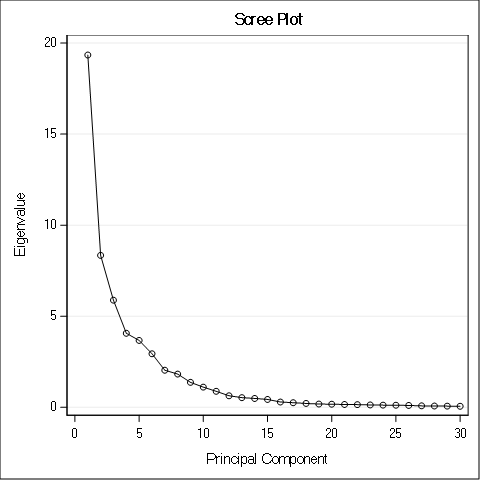
\includegraphics[height=3.95833in]{images/scree.png}

There are a number of options available for determining how many
components should be retained. One possibility is to simply set an
arbitrary threshold on the desired amount of retained variability.
Alternatively, we can take a more informed approach and leverage the
Scree plot above to assess any substantial drop-offs in explained
variance over each component. Such a method may motivate us to retain
the first four components, as the amount of explained variance does seem
to level off beyond this level. For this assessment however, we allow
the first fifteen components to be retained in an attempt to capture the
maximum amount of explained variance.

\subsection{8.2 Model 4: PCA Model}\label{model-4-pca-model}

Parameter estimates for the PCA Model (Model\_PCA) are shown below.

\paragraph{Table 8.2.1: PCA Model Parameter Estimates (Training
Set)}\label{table-8.2.1-pca-model-parameter-estimates-training-set}

\begin{longtable}[]{@{}lllllll@{}}
\toprule
Variable & DF & Parameter Estimate & Standard Error & t Value &
\$\text{Pr} \textgreater{} & t\tabularnewline
\midrule
\endhead
Intercept & 1 & 80.64409 & 0.33936 & 237.63 & \textless{}.0001 &
0\tabularnewline
Prin1 & 1 & 0.24426 & 0.07745 & 3.15 & 0.0016 & 1.0086\tabularnewline
Prin2 & 1 & 1.74522 & 0.11696 & 14.92 & \textless{}.0001 &
1.01017\tabularnewline
Prin3 & 1 & 1.449 & 0.14212 & 10.2 & \textless{}.0001 &
1.01549\tabularnewline
Prin4 & 1 & 1.19577 & 0.16954 & 7.05 & \textless{}.0001 &
1.00413\tabularnewline
Prin5 & 1 & 0.01219 & 0.17527 & 0.07 & 0.9445 & 1.00323\tabularnewline
Prin6 & 1 & -2.26033 & 0.19259 & -11.74 & \textless{}.0001 &
1.00547\tabularnewline
Prin7 & 1 & 0.54104 & 0.23257 & 2.33 & 0.0201 & 1.00847\tabularnewline
Prin8 & 1 & -1.3535 & 0.25583 & -5.29 & \textless{}.0001 &
1.01993\tabularnewline
Prin9 & 1 & 2.1215 & 0.29347 & 7.23 & \textless{}.0001 &
1.02084\tabularnewline
Prin10 & 1 & -0.27843 & 0.31722 & -0.88 & 0.3802 & 1.0171\tabularnewline
Prin11 & 1 & -0.10821 & 0.35374 & -0.31 & 0.7597 &
1.01481\tabularnewline
Prin12 & 1 & -1.41118 & 0.42144 & -3.35 & 0.0008 &
1.01014\tabularnewline
Prin13 & 1 & -1.17669 & 0.46832 & -2.51 & 0.0121 &
1.01585\tabularnewline
Prin14 & 1 & -1.6239 & 0.47863 & -3.39 & 0.0007 & 1.02133\tabularnewline
Prin15 & 1 & -0.9432 & 0.5163 & -1.83 & 0.0679 & 1.04349\tabularnewline
\bottomrule
\end{longtable}

For Model\_PCA, the majority of coefficient estimates have significant
p-values at the 95\% level, allowing us to reject the null hypothesis
and conclude that each have non-zero coefficients. The only exceptions
to this are components five, ten, eleven and fifteen. The greatest
improvement however is in the reported VIF value for each coefficient
estimate. The VIF for all variables are close to one, which suggests no
correlation between predictors.

Goodness-of-fit information for Model\_PCA is shown below.

\paragraph{Table 8.2.2: PCA Model Analysis of Variance (Training
Set)}\label{table-8.2.2-pca-model-analysis-of-variance-training-set}

\begin{longtable}[]{@{}llllll@{}}
\toprule
Source & DF & Sum of Squares & Mean Square & F Value & Pr \textgreater{}
F\tabularnewline
\midrule
\endhead
Model & 15 & 122014 & 8134.27504 & 45.34 &
\textless{}.0001\tabularnewline
Error & 1546 & 277365 & 179.40795 & &\tabularnewline
Corrected Total & 1561 & 399379 & & &\tabularnewline
\bottomrule
\end{longtable}

The model has reported a large F-value suggesting that the observations
and regression differ from the grand mean. Likewise, the F-value has a
highly significant p-value under the null hypothesis that there is no
linear relationship between the predictor and response variable.

Model performance statistics over the training set for Model\_PCA are
shown below.

\paragraph{Table 8.2.3: PCA Model Performance Metrics (Training
Set)}\label{table-8.2.3-pca-model-performance-metrics-training-set}

\begin{longtable}[]{@{}llll@{}}
\toprule
Measure & Value & Measure & Value\tabularnewline
\midrule
\endhead
MSE & 179.40795 & R-Square & 0.3055\tabularnewline
MAE & 10.4695 & Adj R-Sq & 0.2988\tabularnewline
Root MSE & 13.39433 & C(p) & 16.0000\tabularnewline
Dependent Mean & 80.57875 & AIC & 8122.1699\tabularnewline
Coeff Var & 16.62265 & BIC & 8124.5009\tabularnewline
\bottomrule
\end{longtable}

The R-square value above suggests that Model\_PCA explains
\textasciitilde{}30\% of the variability in TARGET\_WINS. The adjusted
R-squared value also indicates a similar level of explanatory power. The
adjusted R-squared value for this specification is lower (inferior) than
the other three models and its AIC and BIC are also higher (inferior).

Model performance statistics over the training set for Model\_PCA are
shown below.

\paragraph{Table 8.2.4: PCA Model Performance Metrics (Test
Set)}\label{table-8.2.4-pca-model-performance-metrics-test-set}

\begin{longtable}[]{@{}llll@{}}
\toprule
Measure & Value & Measure & Value\tabularnewline
\midrule
\endhead
MSE & 166.34445 & R-Square & 0.2959\tabularnewline
MAE & 9.90133 & Adj R-Sq & 0.2807\tabularnewline
Root MSE & 12.89746 & C(p) & 16.0000\tabularnewline
Dependent Mean & 81.25490 & AIC & 3667.2573\tabularnewline
Coeff Var & 15.87284 & BIC & 3669.9898\tabularnewline
\bottomrule
\end{longtable}

Again, performance metrics for Model\_PCA have remained fairly
consistent between the training and test sets. This suggests that the
model is able to generalize over the test set of data.

While its performance metrics were found to be generally inferior to the
other three models, we have elected to generate predictions using this
model over the final test set of data. We find that the trade-off in
performance to be acceptable in eliminating the multicollinearity issues
found in the other three specifications.

\newpage

\section*{References}\label{references}
\addcontentsline{toc}{section}{References}

\hypertarget{refs}{}
\hypertarget{ref-Mont2012}{}
D. Montgomery, \& G. Vining, E. Peck. 2012. ``Introduction to Linear
Regression Analysis.'' John Wiley \& Sons Inc.

\hypertarget{ref-Sasi2016}{}
Inc, SAS Institute. 2016. ``SAS/STAT(R) 9.22 User's Guide.''
\url{https://support.sas.com/documentation/cdl/en/statug/63347/HTML/default/viewer.htm\#statug_reg_sect030.htm}.


\end{document}
